\documentclass{homework}
\usepackage{homework}
\title{Week 1}
\date{}
\begin{document}
\maketitle
\section{“抵消现象”:考察$\lim\limits_{x\to0} \frac{1-\cos(x)}{x^2}$的计算值(P7)}
    为了考察计算值与极限值$\frac{1}{2}$的差,做函数$y=|\frac{1-\cos(x)}{x^2}|$,并用双对数坐标轴画出函数图像。代码如下:
    \lstinputlisting[language=Matlab]{prob1.m}
    得到的图像如下:
    \begin{figure}[H]
    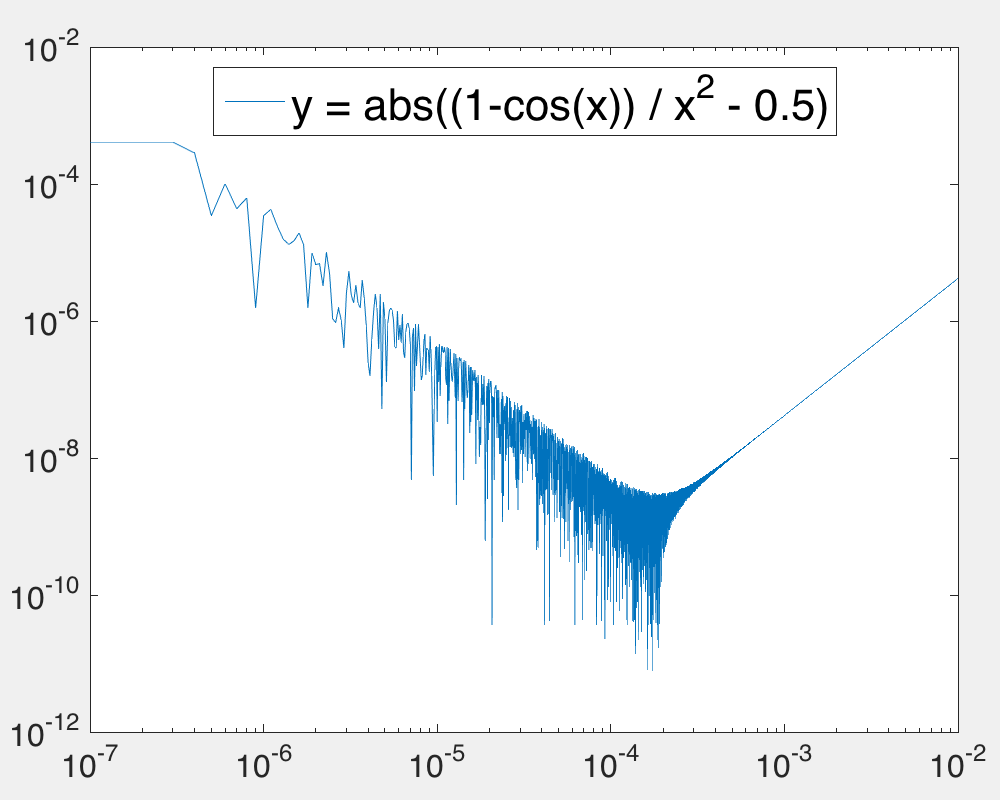
\includegraphics[width=7cm]{fig01.png}
    \centering
    \end{figure}
    可以看出,在$x$从上接近$10^{-4}$时,函数值越来越接近极限值$\frac{1}{2}$,误差一度达到近$10^{-10}$;而当$x$继续趋近0时,误差的数量级开始震荡上升,当$x$小到$10^{-7}$级别时,误差竟然已经扩大到了$10^{-3}$级别。可见在求无穷小之比的未定型数值时,过小的量反而会放大误差,这是因为用于计算的数值大小不断接近浮点数的舍入误差大小(机器精度)造成的。
    \clearpage
\section{考察三种迭代矩阵$\bm{A}$的条件数$\operatorname{cond}(\bm{A})$随阶数增长的变化(P9/图1.3)}
    $$\hspace{-2em}
    \bm{A}_1=\begin{pmatrix}
    1 & & & & \\
    & 1 & & & \\
    2 & -3 & 1 & & \\
    & \ddots & \ddots & \ddots & \\
    & & 2 & -3 & 1
    \end{pmatrix}_{N\times N}
    \hspace{-2em}
    \bm{A}_2=\begin{pmatrix}
    1 & & & & -1 \\
    & 1 & & & \\
    2 & -3 & 1 & & \\
    & \ddots & \ddots & \ddots & \\
    & & 2 & -3 & 1
    \end{pmatrix}_{N\times N}
    \hspace{-2em}
    \bm{A}_3=\begin{pmatrix}
    1 & & & & \\
    & 1 & & & \\
    1 & -2 & 1 & & \\
    & \ddots & \ddots & \ddots & \\
    & & 1 & -2 & 1
    \end{pmatrix}_{N\times N}$$
    运用Matlab计算以上三种迭代矩阵的条件数:
    \lstinputlisting[language=Matlab]{prob2.m}
    其条件数随阶数增长的趋势如图:
    \begin{figure}[H]
    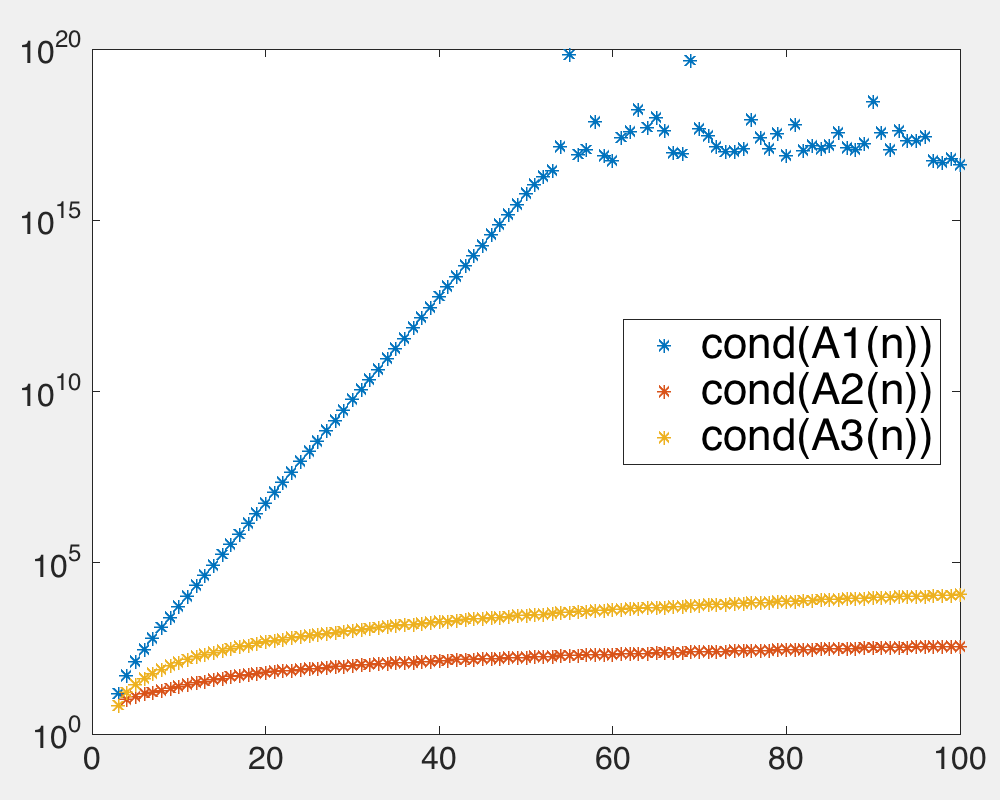
\includegraphics[width=7cm]{fig02.png}
    \centering
    \end{figure}
    可以看出$\bm{A}_1$条件数随阶数增长速度远高于$\bm{A}_3$的增长,呈指数增长趋势,到60阶左右时就达到$10^{16}$数量级且开始出现计算偏差。而再矩阵的右上角加上一个-1,也就是限定了迭代最后一项和第一项的关系,这时$\bm{A}_2$的条件数增长速度一下就降低了。
    \clearpage
\section{证明不动点迭代的误差估计式(P17/式1.2.8)}
    \begin{proof}
    如果映射$G(x)$是一个压缩映射,则存在常数$\alpha \in[0,1)$,有$$\norm{G(x)-G(y)}\leqslant \alpha \norm{x-y},$$由单步迭代,上式等价于$$\norm{x_{n+1}-x_n} \leqslant \alpha \norm{x_n-x_{n-1}},$$反复运用上式,得到
    \begin{align*}
    \norm{x_{n+1}-x_n} & \leqslant \alpha^2 \norm{x_{n-1}-x_{n-2}}  \\
    & \leqslant \alpha^3 \norm{x_{n-2}-x_{n-3}} \\
    & \cdots \\
    & \leqslant \alpha^n \norm{x_1-x_0} \\
    \end{align*}
    所以当$m>n$时,
    \begin{align*}
    \norm{x_m-x_n} & \leqslant \norm{x_m-x_{m-1}} + \norm{x_{m-1}-x_{m-2}} + \cdots + \norm{x_{n+1}-x_n}  \\
    & \leqslant ( \alpha^{m-n-1} + \alpha^{m-n-2} + \cdots + \alpha + 1 ) \norm{x_{n+1}-x_n} \\
    & = \frac{1-\alpha^{m-n}}{1-\alpha}\norm{x_{n+1}-x_n} \\
    & \leqslant \frac{1-\alpha^{m-n}}{1-\alpha} \alpha^n \norm{x_1-x_0}
    \end{align*}
    因为$\alpha \in [0,1)$,所以令$m\to\infty$,有$\alpha^{m-n} \to 0$,此时$x_m\to x^*$,便得到了不动点迭代的误差估计式:$$\norm{x^*-x_n} \leqslant \frac{\alpha^n}{1-\alpha} \norm{x_1-x_0}.$$
    \end{proof}
    \clearpage
\section{比较不动点迭代和Newton-Raphson迭代,实现数值例子并定性说明理由(P24/2)}
    取$G(x)=e^{-x}$和$F(x)=x-e^{-x}$,取$x_0=1$为迭代初始值,则由不动点迭代和Newton-Raphson迭代得到的结果与其误差如下表:
    \begin{table}[H]
    \centering
    {\rowcolors{3}{}{black!5}
    \begin{tabular}{|c||c|c|c||c|c|c|}
        \hline
        \multirow{2}*{n}
        & \multicolumn{3}{c||}{Fixed-point Iteration}
        & \multicolumn{3}{c|}{Newton-Raphson Iteration} \\\cline{2-7}
        & $x_n$ & $\frac{\abs{x_n-x_{n-1}}}{\abs{x_n}}$ & $\frac{\abs{x_n-x^*}}{\abs{x^*}}$
        & $x_n$ & $\frac{\abs{x_n-x_{n-1}}}{\abs{x_n}}$ & $\frac{\abs{x_n-x^*}}{\abs{x^*}}$ \\\hline
         0 & 1.000000 &    -    & 1.8e\Plus00 & 1.000000 &    -    & 1.8e\Plus00 \\
         1 & 0.367879 & 1.7e\Plus00 & 3.5e\Minus01 & 0.537883 & 8.6e\Minus01 & 5.2e\Minus02 \\
         2 & 0.692201 & 4.7e\Minus01 & 2.2e\Minus01 & 0.566987 & 5.1e\Minus02 & 2.8e\Minus04 \\\hline
         3 & 0.500474 & 3.8e\Minus01 & 1.2e\Minus01 & 0.567143 & 2.8e\Minus04 & 7.8e\Minus09 \\
         4 & 0.606244 & 1.7e\Minus01 & 6.9e\Minus02 & 0.567143 & 7.8e\Minus09 & 2.0e\Minus16 \\
         5 & 0.545396 & 1.1e\Minus01 & 3.8e\Minus02 & 0.567143 & 2.0e\Minus16 & 0.0e\Plus00 \\\hline
         6 & 0.579612 & 5.9e\Minus02 & 2.2e\Minus02 & 0.567143 & 2.0e\Minus16 & 2.0e\Minus16 \\
         7 & 0.560115 & 3.5e\Minus02 & 1.2e\Minus02 & 0.567143 & 2.0e\Minus16 & 0.0e\Plus00 \\
         8 & 0.571143 & 1.9e\Minus02 & 7.1e\Minus03 & 0.567143 & 2.0e\Minus16 & 2.0e\Minus16 \\\hline
         9 & 0.564879 & 1.1e\Minus02 & 4.0e\Minus03 & 0.567143 & 2.0e\Minus16 & 0.0e\Plus00 \\
        10 & 0.568429 & 6.2e\Minus03 & 2.3e\Minus03 & 0.567143 & 2.0e\Minus16 & 2.0e\Minus16 \\
        11 & 0.566415 & 3.6e\Minus03 & 1.3e\Minus03 & 0.567143 & 2.0e\Minus16 & 0.0e\Plus00 \\\hline
        12 & 0.567557 & 2.0e\Minus03 & 7.3e\Minus04 & 0.567143 & 2.0e\Minus16 & 2.0e\Minus16 \\
        13 & 0.566909 & 1.1e\Minus03 & 4.1e\Minus04 & 0.567143 & 2.0e\Minus16 & 0.0e\Plus00 \\
        14 & 0.567276 & 6.5e\Minus04 & 2.3e\Minus04 & 0.567143 & 2.0e\Minus16 & 2.0e\Minus16 \\\hline
        15 & 0.567068 & 3.7e\Minus04 & 1.3e\Minus04 & 0.567143 & 2.0e\Minus16 & 0.0e\Plus00 \\
        16 & 0.567186 & 2.1e\Minus04 & 7.5e\Minus05 & 0.567143 & 2.0e\Minus16 & 2.0e\Minus16 \\
        17 & 0.567119 & 1.2e\Minus04 & 4.3e\Minus05 & 0.567143 & 2.0e\Minus16 & 0.0e\Plus00 \\\hline
        18 & 0.567157 & 6.7e\Minus05 & 2.4e\Minus05 & 0.567143 & 2.0e\Minus16 & 2.0e\Minus16 \\
        19 & 0.567135 & 3.8e\Minus05 & 1.4e\Minus05 & 0.567143 & 2.0e\Minus16 & 0.0e\Plus00 \\
        20 & 0.567148 & 2.2e\Minus05 & 7.8e\Minus06 & 0.567143 & 2.0e\Minus16 & 2.0e\Minus16 \\\hline
        21 & 0.567141 & 1.2e\Minus05 & 4.4e\Minus06 & 0.567143 & 2.0e\Minus16 & 0.0e\Plus00 \\
        22 & 0.567145 & 6.9e\Minus06 & 2.5e\Minus06 & 0.567143 & 2.0e\Minus16 & 2.0e\Minus16 \\
        23 & 0.567142 & 3.9e\Minus06 & 1.4e\Minus06 & 0.567143 & 2.0e\Minus16 & 0.0e\Plus00 \\\hline
        24 & 0.567144 & 2.2e\Minus06 & 8.1e\Minus07 & 0.567143 & 2.0e\Minus16 & 2.0e\Minus16 \\
        25 & 0.567143 & 1.3e\Minus06 & 4.6e\Minus07 & 0.567143 & 2.0e\Minus16 & 0.0e\Plus00 \\
        26 & 0.567143 & 7.2e\Minus07 & 2.6e\Minus07 & 0.567143 & 2.0e\Minus16 & 2.0e\Minus16 \\\hline
        % 27 & 0.567143 & 4.1e\Minus07 & 1.5e\Minus07 & 0.567143 & 2.0e\Minus16 & 0.0e\Plus00 \\
        % 28 & 0.567143 & 2.3e\Minus07 & 8.3e\Minus08 & 0.567143 & 2.0e\Minus16 & 2.0e\Minus16 \\
        % 29 & 0.567143 & 1.3e\Minus07 & 4.7e\Minus08 & 0.567143 & 2.0e\Minus16 & 0.0e\Plus00 \\\hline
    \end{tabular}
    } % end of rowcolor
    \end{table}
    由Newton-Raphson迭代在第四次迭代以后就已经达到了机器精度,故表中精确值$x^*$用牛顿迭代的$x_{29}$代替。而不动点迭代在迭代24次以后也没有达到这个精度,这是由于不动点迭代误差有$\abs{\epsilon_{n+1}}\leqslant\alpha\abs{\epsilon_n}$,在本例中$\alpha=\abs{G'(x^*)}\approx 0.567$,而牛顿迭代误差有$\abs{\epsilon_{n+1}}\approx\rho\abs{\epsilon_n}^2$,在本例中$\rho=\frac{1}{2}\abs{(F'(x^*))^{-1}}\abs{F''(x^*)}\approx 0.181$。$\alpha$与$\rho$属同一数量级,而不动点迭代误差是一阶减少,但牛顿迭代误差是二阶的,故收敛较快。这一结果也与表中数据相吻合。
    \clearpage
    附数据生成代码:
    \lstinputlisting[language=Matlab]{prob4.m}
\section{证明范数等价关系(P34/1)}
    对于$n$维向量$\bm{x}$,当$1\leqslant p\leqslant q$时,有$$\bignorm{\bm{x}}_{\ell_q}\leqslant\bignorm{\bm{x}}_{\ell_p}\leqslant n^{\frac{1}{p}-\frac{1}{q}}\bignorm{\bm{x}}_{\ell_q}.$$
    \begin{proof}
    由幂平均不等式,当$0<p\leqslant q$时,有$$\bigps{\frac{\abs{x_1}^p+\abs{x_2}^p+\cdots+\abs{x_n}^p}{n}}^{\frac{1}{p}}\leqslant\bigps{\frac{\abs{x_1}^q+\abs{x_2}^q+\cdots+\abs{x_n}^q}{n}}^{\frac{1}{q}},$$整理后即得到右边的不等式$$\bignorm{\bm{x}}_{\ell_p}\leqslant n^{\frac{1}{p}-\frac{1}{q}}\bignorm{\bm{x}}_{\ell_q}.$$
    另外,将$\bm{x}$按$q$范数单位化,即令$\bm{\hat{x}}=\bignorm{\bm{x}}_{\ell_q}^{-1}\bm{x},$此时$\bignorm{\bm{\hat{x}}}_{\ell_q}=1,$每个分量$\hat{x}_i=\frac{x_i}{\bignorm{\bm{x}}_{\ell_q}}\leqslant 1,$所以$$\bigps{\frac{x_i}{\bignorm{\bm{x}}_{\ell_q}}}^p\geqslant\bigps{\frac{x_i}{\bignorm{\bm{x}}_{\ell_q}}}^q\quad(p<q),$$求和后仍有$$\sum_{i=1}^n\bigps{\frac{x_i}{\bignorm{\bm{x}}_{\ell_q}}}^p\geqslant\sum_{i=1}^n\bigps{\frac{x_i}{\bignorm{\bm{x}}_{\ell_q}}}^q=1$$所以$$\bignorm{\bm{\hat{x}}}_{\ell_p}=\bigps{\sum_{i=1}^n\bigps{\frac{x_i}{\bignorm{\bm{x}}_{\ell_q}}}^p}^{\frac{1}{p}}\geqslant 1=\bignorm{\bm{\hat{x}}}_{\ell_q}.$$
    最后,由范数的齐次性$\bignorm{a\bm{x}}=a\bignorm{\bm{x}}$,取$a=\bignorm{\bm{\hat{x}}}_{\ell_q}^{-1}$便得到了左边的不等式$$\bignorm{\bm{x}}_{\ell_q}\leqslant\bignorm{\bm{x}}_{\ell_p}.$$
    \end{proof}
\end{document}
